\documentclass[tikz,border=6pt]{standalone}
\usepackage{tikz}
\usetikzlibrary{positioning, shapes, arrows.meta, shadows, calc}

\begin{document}
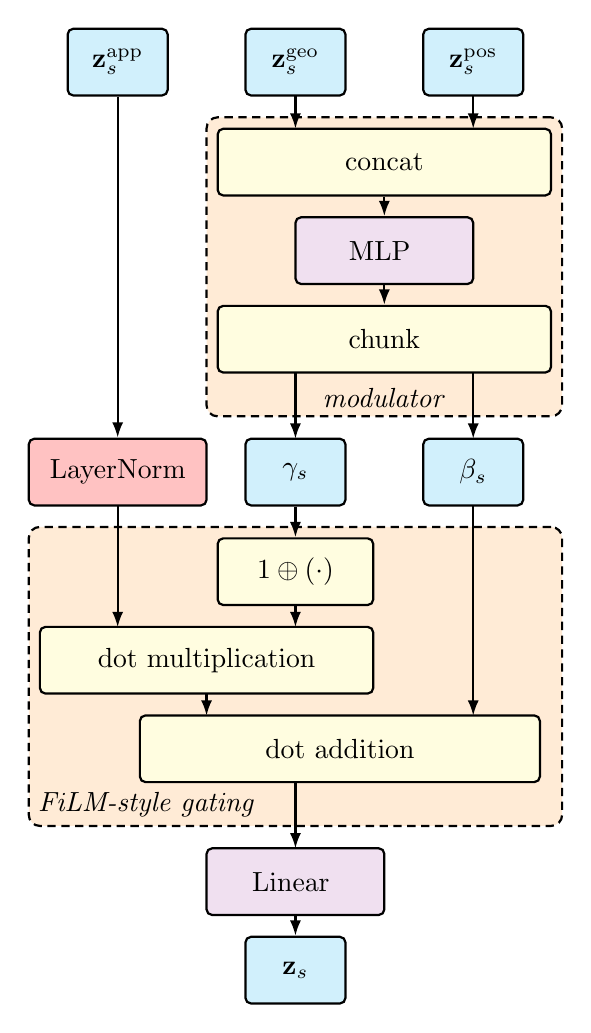
\begin{tikzpicture}[
    io/.style={
        draw, rounded corners=2px, fill=cyan!18, minimum width=36px, minimum height=24px, align=center},
    layer/.style={
        draw, rounded corners=2px, fill=red!24, minimum width=56px, minimum height=24px, align=center},
    gcn/.style={
        draw, rounded corners=2px, fill=green!12, minimum width=144px, minimum height=24px, align=center},
    dropout/.style={
        draw, rounded corners=2px, fill=violet!18, minimum width=64px, minimum height=24px, align=center},
    opr/.style={
        draw, rounded corners=2px, minimum height=24px, ,minimum width=120px, fill=yellow!12,},
    mlp/.style={
        draw, rounded corners=2px, fill=violet!12, minimum height=24px, align=center},
    > = {Latex[length=5.5px, width=4px]},
    thick,
]

\node[layer, minimum width=128px, minimum height=32+32+32+12px, densely dashed, rounded corners=4pt, fill=orange!16] at (32px, -48-32+6px) (modulator) {};

\node[anchor=south] at (modulator.south) {\textit{modulator}};


\node[io] at (-64px, 0px) (app) { $\mathbf{z}_s^{\mathrm{app}}$};

\node[io] at (0px, 0px) (geo) { $\mathbf{z}_s^{\mathrm{geo}}$};

\node[io] at (64px, 0px) (pos) { $\mathbf{z}_s^{\mathrm{pos}}$};

\draw[->] ($ (geo) + (0, -12px) $) -- ($ (geo) + (0,-12-12px) $);

\draw[->] ($ (pos) + (0, -12px) $) -- ($ (pos) + (0,-12-12px) $);

\node[opr] at (32px, -36px) (concat) { $\mathrm{concat}$ };

\node[mlp, minimum width=64px] at (32px, -36-32px) (mlp1) { $\mathrm{MLP}$ };

\draw[->] (concat) -- (mlp1);

\node[opr] at (32px, -36-32-32px) (chunk) { $\mathrm{chunk}$ };

\draw[->] (mlp1) -- (chunk);

\node[io] at (0, -48-32-32-36px) (gamma) { $\gamma_s$};

\node[io] at (64px, -48-32-32-36px) (beta) { $\beta_s$};

\node[layer, minimum width=192px, minimum height=32+32+32+12px, densely dashed, rounded corners=4pt, fill=orange!16] at (0px, -48-32-32-36-48-32+6px) (gate) {};

\node[anchor=south west] at (gate.south west) {\textit{FiLM-style gating}};

\draw[->] ($ (gamma) + (0, 12+24px) $) -- ($ (gamma) + (0,12px) $);

\draw[->] ($ (beta) + (0, 12+24px) $) -- ($ (beta) + (0,12px) $);

\node[opr, minimum width=56px] at (0px, -48-32-32-36-36px) (add1) {$1\oplus(\cdot)$};

\draw[->] (gamma) -- (add1);

\node[layer, minimum width=64px] at (-64px, -48-32-32-36px) (ln) {$\mathrm{LayerNorm}$};

\draw[->] (app) -- (ln);

\node[opr] at (-32px, -48-32-32-36-36-32px) (mul) {dot multiplication};

\draw[->] ($ (ln) + (0, -12px) $) -- ($ (ln) + (0, -12-36-8px) $);

\draw[->] ($ (add1) + (0, -12px) $) -- ($ (add1) + (0, -12-8px) $);

\draw[->] ($ (mul) + (0, -12px) $) -- ($ (mul) + (0, -12-8px) $);

\draw[->] ($ (beta) + (0, -12px) $) -- ($ (beta) + (0, -16-32-32-8px) $);

\node[opr, minimum width=144px] at (16px, -48-32-32-36-36-32-32px) (add) {dot addition};

\node[mlp, minimum width=64px] at (0, -48-32-32-36-48-32-32-36px) (mlp2) { $\mathrm{Linear}$ };

\draw[->] ($ (mlp2) + (0, 12+24px) $) -- ($ (mlp2) + (0, 12px) $);

\node[io] at (0, -48-32-32-36-48-32-32-36-32px) (out) { $\mathbf{z}_s$};

\draw[->] (mlp2) -- (out);

\end{tikzpicture}
\end{document}
